In this section we introduce a metalanguage for describing the semantics of
processor instructions by following a few examples. We will use the metalanguage
to describe the semantics of a part of a simple generic instruction set
architecture. The later sections will introduce a formal definition of the
metalanguage, instruction semantics and present a method for
extracting static data dependencies of instructions with certain properties from
the semantic definitions leading to a construction of a concurrency oracle.
Fig.~\ref{fig-example} shows three example dependency graphs that can be
automatically produced by the presented method.

% Unconstrained semantics
\vspace{-2mm}
\subsubsection{Load} Loading a data word from memory to a register is one of the
simplest processor instructions. Here is
how\footnote{We use Haskell throughout the paper, not only because it is one of
the most popular functional programming languages, but also because it provides
support for \emph{higher-rank polymorphism}~\cite{jones2007practical}, which is
essential for the presented approach.} we encode its semantics in our metalanguage:

\vspace{-1mm}
\begin{minted}[xleftmargin=10pt]{haskell}
load reg addr = \read write -> Just $
    write (Reg reg) (read (Addr addr))
\end{minted}
\vspace{-1mm}

\noindent
In this definition we use two metalanguage terms \hs{read} and \hs{write} to
specify the behaviour of the instruction, specifically to \emph{read} the memory
location at \emph{address} \hs{addr}, and \emph{write} the result into the
\emph{register} \hs{reg}. Crucially, \hs{read} and \hs{write} are
\emph{polymorphic over the computational context} \hs{f} and have the following
types:

\vspace{-1mm}
\begin{minted}[xleftmargin=10pt]{haskell}
read  :: forall f. Key -> f Value
write :: forall f. Key -> f Value -> f ()
\end{minted}
\vspace{-1mm}

\noindent
Here \hs{Key} is used to identify a particular component of the processor state,
such as a memory location or a register, and \hs{Value} is the type of data the
processor operates on, e.g. \hs{Value} for a 64-bit processor.

The~\hs{read} term queries the microarchitectural state for the value of a key
and returns it wrapped in a context~\hs{f}, which in this case captures the
effect of reading from the state. The~\hs{write} term takes a key and a value,
and modifies the microarchitectural state, returning no information (the
\emph{unit} \hs{()}), but capturing the effect of writing in the context \hs{f}.

% which is, in fact, the reason for the
% metalanguage to be~\emph{polymorphic}. In this case the context~\hs{f} may be any
% type constructor of kind~\hs{* -> *}. However, not every instruction semantics may
% be expressed in an unconstrained context. Let us consider semantics of some other
% instructions to elaborate more on the nature of~\hs{f}.

\begin{figure}
\vspace{-6mm}
\centerline{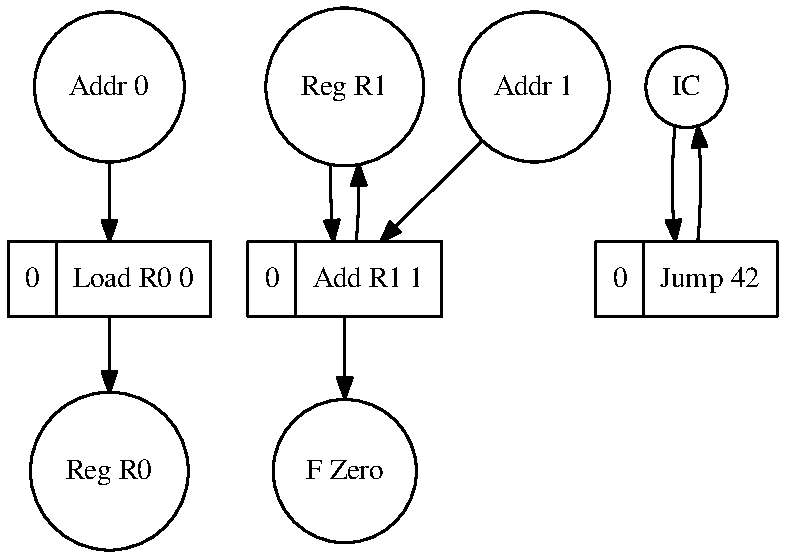
\includegraphics[scale=0.7]{img/loadJumpAdd.pdf}}
\vspace{-6mm}
\caption{Static data dependencies of~\hs{Load R0 0}, \hs{Add R1 1} and
\hs{Jump 42} instructions\protect\footnotemark. The `0' inside the instruction
boxes corresponds to the address of an instruction in the program and will be
useful for visualising blocks of instructions.\label{fig-example}}
\vspace{-6mm}
\end{figure}
\footnotetext{We used the \textsf{algebraic-graphs} Haskell
library~\cite{2017_mokhov_alga} to export dependency graphs into
the DOT format, and then applied GraphViz~\cite{graphviz} for automated layout.}

%Functorial semantics
\subsubsection{Jump}

Another simple instruction is the unconditional control flow transfer:

\begin{minted}[xleftmargin=10pt]{haskell}
jump offset = \read write -> Just $
    write IC ((+ offset) <$> (read IC))
\end{minted}

\noindent
This instruction adds an \hs{offset} to the \emph{instruction counter}~\hs{IC}
to transfer the control to another instruction in the program. This definition
has a crucial difference from~\hs{load}: it uses the function~\hs{<$>} of
the~\hs{Functor} type class\footnote{Function~\hs{<$>} (pronounced ``fmap'') of
type \hs{Functor f => (a -> b) -> f a -> f b} transforms the values in a
computational context \hs{f} using a pure function.}, thus restricting~\hs{f} of
the \hs{read} and \hs{write} terms to be a~\hs{Functor}:

\vspace{-1mm}
\begin{minted}[xleftmargin=10pt]{haskell}
read  :: forall f. Functor f => Key -> f Value
write :: forall f. Functor f => Key -> f Value -> f ()
\end{minted}

In this definition the functorial constraint is required to apply the addition
function \hs{(+ offset) :: Value -> Value} to the instruction counter value
enclosed in a computational context~\hs{f}. We therefore say that \hs{jump} has
\emph{functorial semantics}, whereas \hs{load} has \emph{unconstrained semantics},
since the \hs{read} and \hs{write} terms had no constraint.

Later in the paper we will instantiate~\hs{f} with an appropriate context for
data dependency tracking. As it turns out, instructions that have unconstrained
or functorial semantics can have at most one read dependency: there is no way
to combine multiple read results. To do that, we need \emph{applicative
semantics}, as demonstrated by the next example.

% Applicative semantics
\vspace{-3mm}
\subsubsection{Add}

The~\hs{add} instruction performs the addition of the values of a register and
a memory cell, writing the result back into the same register. If the result of
the addition is equal to zero, the instruction sets the~\hs{Zero} flag of the
processor to~\hs{True}, and to~\hs{False} otherwise.

The semantics definition is a bit more involved than the previous ones, because
the~\hs{Functor} context is not expressive enough and a more powerful
abstraction is needed. The following definition of~\hs{add} requires
\hs{f} to be at least an~\hs{Applicative}:

\begin{minted}[xleftmargin=10pt]{haskell}
add reg addr = \read write -> Just $
    let result = (+)    <$> read (Reg reg) <*> read (Addr addr)
        isZero = (== 0) <$> result
    in  write (Reg reg) result *>
        write (Flag Zero) (boolToValue <$> isZero)
\end{minted}

\noindent
Let us elaborate on what is going on here. The definition may be broken down
into three parts: reading data, processing it, and writing data back in the
processor state.

The first~\hs{let}-binding uses~\hs{Applicative} notation to read the values
from the register \hs{reg} and memory address \hs{addr} and add them up. Note
that this notation is~\emph{declarative}, hence it rather states that
the~\hs{result} is supposed to be a sum of values of two entities than performs
actual computation. This intuition is very important for understanding the
static dependency tracking of instructions: keys \hs{Reg}~\hs{reg} and
\hs{Addr}~\hs{addr} are declared as static input dependencies of the~\hs{add}
instruction. However, since the semantics may be executed in
any~\hs{Applicative} context, this dependency-tracking interpretation does not
prevent other possible interpretations of the very same definition of the
semantics. For instance, in a simulation context, the~\hs{result} will be
computed based on concrete data values read from the current processor state.

The second line of the~\hs{let}-binding is quite similar to the expression in the
semantics of the~\hs{jump} instruction. The type of the~\hs{result} is~\hs{f Value},
hence the zero testing function~\hs{(== 0)} of type~\hs{Value -> Bool}
must be mapped over the context~\hs{f} with the operator~\hs{<$>} to obtain the
value of type \hs{f Bool}.

The last two lines of the definition perform two~\hs{write} operations chained
with the applicative operator~\hs{*>} of
type~\hs{Applicative f => f a -> f b -> f b}.
This declares the keys~\hs{Reg}~\hs{reg} and~\hs{Flag}~\hs{Zero} to be output
dependencies of the computation and that the writes must be both performed.
The the \hs{read} and \hs{write} terms now have the following types:

\begin{minted}[xleftmargin=10pt]{haskell}
read  :: forall f. Applicative f => Key -> f Value
write :: forall f. Applicative f => Key -> f Value -> f ()
\end{minted}

An interesting feature of the~\hs{Applicative} notation is that it does not
specify the exact order of performing actions. This is useful in
embedded domain-specific languages with concurrency, for instance
Facebook's Haxl~\cite{Marlow:2014:NFA:2692915.2628144}. This insight can also
be used to extract concurrency from instruction descriptions.

\hs{Applicative} functors are powerful enough to express the semantics of a
large class of instructions. In this paper we exploit their features to not only
specify the execution semantics but also automatically track static data dependencies
of instructions. However not every instruction can be expressed with applicative
semantics. If the behaviour depends on the actual data values,
i.e. when \emph{dynamic data dependencies} emerge, a more powerful
\emph{monadic semantics} is required.

%Monadic semantics
\subsubsection{Indirect load}

The indirect memory access instruction looks up a value in a memory cell and uses
it as the effective address in the regular load instruction. Since the effective
address can not be determined statically in the general case, this instruction
has a dynamic data dependency. The polymorphic computational metalanguage requires
the context~\hs{f} to be a \hs{Monad} in order to be able to encode such behaviour.
Consider the definition of the semantics of the \hs{loadMI} instruction, which
uses Haskell's monadic \hs{do}-notation:

\begin{minted}[xleftmargin=10pt]{haskell}
loadMI reg addr read write = Just $ do
    addr' <- read (Addr addr)
    write (Reg reg) (read (Addr addr'))
\end{minted}

\noindent
The first line extracts the effective address from the monadic context~\hs{f}
and binds the identifier~\hs{addr'} to it. Here is the catch: expressions
on left-hand-side and right-hand-side of the~\hs{<-} symbol have different types.
The~\hs{read (Addr addr)} is of type~\hs{Monad f => f Value} and the
identifier~\hs{addr'} has type \hs{Value}. The main feature of~\hs{Monad} is the
ability to extract a value from an effectful context and pass it in the further
computation as if it was pure. This gives us a possibility to pass the~\hs{addr'}
as an argument to the next~\hs{read} operation.

Monadic semantics is more powerful than unconstrained, functorial and applicative ones,
but we are no longer able to extract all the dependencies of the computation if
\hs{f} is restricted to~\hs{Monad}, since some of them will not be static.
Therefore, concurrency oracles can not be built for~\hs{Monad}-flavoured
computations, or at least, they can no longer be exact and must be approximate
(for example, one might conservatively say that \hs{loadMI} has a read
dependency on every possible memory address, but no register read dependencies).

We have given examples of four types of semantic computations: unrestricted,
functorial, applicative and monadic. In every definition we used
functions~\hs{read} and~\hs{write} with appropriate constraints on the
context~\hs{f}. To recap, here are the four different types for the \hs{read}
function:

\begin{minted}[xleftmargin=10pt]{haskell}
read :: forall f.                  Key -> f Value
read :: forall f.     Functor f => Key -> f Value
read :: forall f. Applicative f => Key -> f Value
read :: forall f.       Monad f => Key -> f Value
\end{minted}

\noindent
One can clearly see a pattern, and Haskell's type system is powerful enough to
abstract over it. Generic \hs{read} and \hs{write} may be assigned the
following types:

\begin{minted}[xleftmargin=10pt]{haskell}
read  :: forall f. c f => Key -> f Value
write :: forall f. c f => Key -> f Value -> f ()
\end{minted}

\noindent
Here, the variable~\hs{c} must have the kind~\hs{* -> Constraint}. This allows
to instantiate \hs{c} with \hs{NoConstraint}, \hs{Functor}, \hs{Applicative},
\hs{Monad} or any other suitable constraint, thus making the metalanguage
polymorphic in the computational context.

The next section will present a formal definition of the metalanguage, instruction
and program semantics. The section~\ref{sec:oracles} will describe the construction
of concurrency oracles for programs comprising unrestricted, functorial,
applicative, but not monadic instructions.
